
%(BEGIN_QUESTION)
% Copyright 2007, Tony R. Kuphaldt, released under the Creative Commons Attribution License (v 1.0)
% This means you may do almost anything with this work of mine, so long as you give me proper credit

Her vises responsen til en regulator med proporsjonal + integralvirkning på en trinnendring i setpunktet (med konstant prosessvariabel). Beregn regulatorens proporsjonal- og integralkonstanter ut fra grafen. Oppgi svaret for integralkonstanten både i enheten ``repetisjoner per minutt'' og ``minutter per repetisjon.'' Bestem også om regulatoren er direkte- eller reversvirkende, og marker hvilke deler av utgangskurven som tilsvarer proporsjonalvirkning og integralvirkning.
  
$$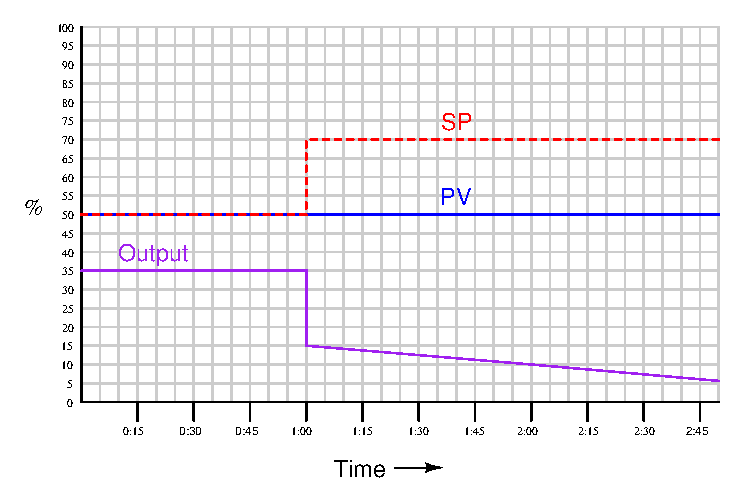
\includegraphics[width=15.5cm]{i01602x01.eps}$$

Tidsskalaen i diagrammet er minutter:sekunder, og PI-algoritmen er som følger:

$$m = K_p \left( e + {1 \over \tau_i} \int e \> dt \right) + b$$

\noindent
Der,

$m$ = regulatorutgang (manipulert variabel)

$K_p$ = forsterkning

$e$ = avvikssignal (SP$-$PV eller PV$-$SP)

$\tau_i$ = integraltidskonstant

$b$ = bias

\vskip 10pt

\vskip 20pt \vbox{\hrule \hbox{\strut \vrule{} {\bf Forslag til sokratisk diskusjon} \vrule} \hrule}

\begin{itemize}
\item{} Når man analyserer utgangstrenden til en PI-regulator, er definisjonen av reset-tidskonstanten som ``antall minutter som trengs for å repetere proporsjonalvirkningen'' spesielt nyttig. Identifiser størrelsen på proporsjonalvirkningen som respons på PV-trinnendringen, og forklar hvordan denne verdien hjelper deg å finne $\tau_i$.
\item{} Hvis du faktisk så denne typen respons i en trend fra en prosessregulator (skrivende trend), hva ville du mistenkt om systemet? Hint: denne trenden er definitivt {\it ikke} normal for et riktig fungerende reguleringssystem!
\end{itemize}

\underbar{file i01602}
%(END_QUESTION)





%(BEGIN_ANSWER)

Regulatorvirkning = {\it direkte}

\vskip 10pt

Forsterkningskonstant = 1, eller 100\% proporsjonalbånd

\vskip 10pt

Integralkonstant = 0.25 repetisjoner per minutt ($K_i$), eller 4 minutter per repetisjon ($\tau_i$)

%(END_ANSWER)





%(BEGIN_NOTES)

Vi vet at denne regulatoren er {\it direktevirkende} fordi utgangen synker når setpunktet (SP) øker. Det betyr at utgangen også ville synke dersom prosessvariabelen (PV) sank.

Regulatorens forsterkning beregnes som forholdet mellom størrelsen på utgangstrinnet og størrelsen på inngangstrinnet: i dette tilfellet gir et utgangstrinn på 20\% et inngangstrinn på 20\%, altså forsterkning 1. Den reciproke verdien gir proporsjonalbånd på 100\%.

Til slutt ser vi at integralvirkningen over ett minutt får utgangen til å drive ytterligere 5\%. Dette er bare 1/4 av proporsjonalresponsen, og derfor blir integralkonstanten 1/4 repetisjon per minutt. Den reciproke verdien er 4 minutter per repetisjon.
 
\vskip 10pt

Hva er galt med dette reguleringssystemet, slik trenden viser? Prosessvariabelen ser helt uresponsiv ut på endringer i utgangssignalet. Det ser ut som om sluttelementet er forbikoblet eller koblet ut på en eller annen måte. Ikke tolke dette som at regulatoren står i manuell modus. En regulator i ``manual'' ville ikke laget endringer i utgangssignalet som respons på endringer i PV eller SP. Med andre ord: en regulator i manuell modus holder et konstant utgangsnivå uansett hva som skjer med PV eller SP.

%INDEX% Control, proportional + integral: graphing controller response

%(END_NOTES)
